% Created by tikzDevice version 0.12.3.1 on 2022-05-25 12:05:34
% !TEX encoding = UTF-8 Unicode
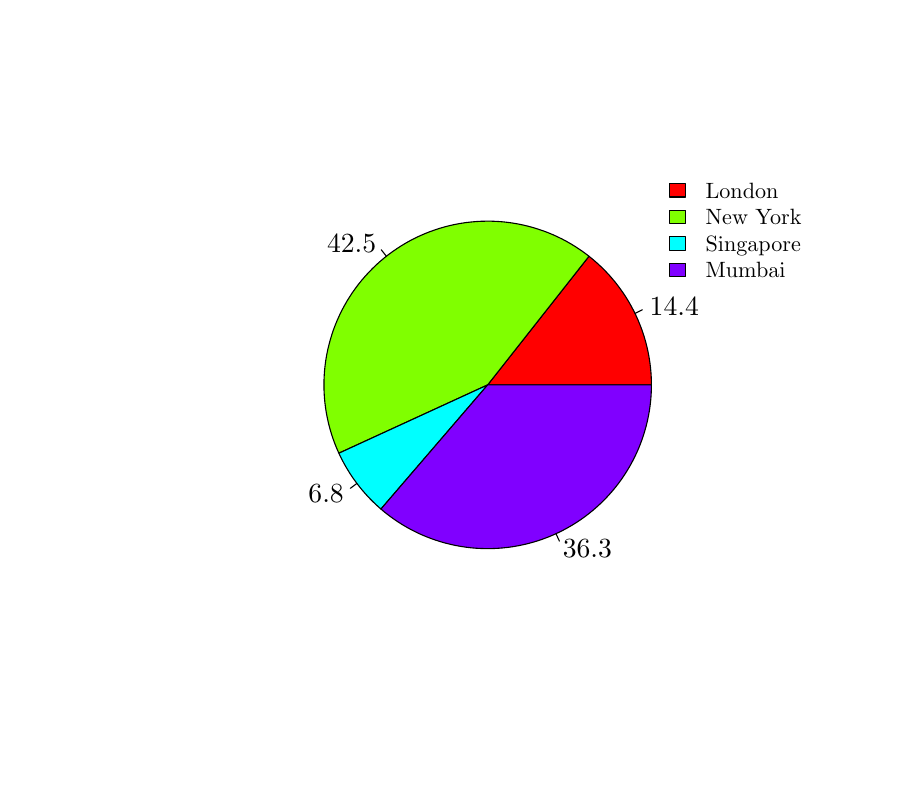
\begin{tikzpicture}[x=1pt,y=1pt]
\definecolor{fillColor}{RGB}{255,255,255}
\path[use as bounding box,fill=fillColor,fill opacity=0.00] (0,0) rectangle (308.44,270.16);
\begin{scope}
\path[clip] ( 49.20, 61.20) rectangle (283.24,220.96);
\definecolor{drawColor}{RGB}{0,0,0}
\definecolor{fillColor}{RGB}{255,0,0}

\path[draw=drawColor,line width= 0.4pt,line join=round,line cap=round,fill=fillColor] (225.39,141.08) --
	(225.36,143.06) --
	(225.26,145.04) --
	(225.09,147.01) --
	(224.86,148.98) --
	(224.56,150.93) --
	(224.20,152.88) --
	(223.77,154.81) --
	(223.28,156.73) --
	(222.73,158.63) --
	(222.11,160.52) --
	(221.42,162.37) --
	(220.68,164.21) --
	(219.88,166.02) --
	(219.01,167.80) --
	(218.09,169.55) --
	(217.11,171.27) --
	(216.07,172.96) --
	(214.97,174.61) --
	(213.82,176.22) --
	(212.62,177.80) --
	(211.36,179.33) --
	(210.06,180.82) --
	(208.70,182.26) --
	(207.30,183.66) --
	(205.85,185.01) --
	(204.36,186.31) --
	(202.83,187.56) --
	(166.22,141.08) --
	cycle;

\path[draw=drawColor,line width= 0.4pt,line join=round,line cap=round] (219.45,166.91) --
	(222.11,168.21);
\end{scope}
\begin{scope}
\path[clip] (  0.00,  0.00) rectangle (308.44,270.16);
\definecolor{drawColor}{RGB}{0,0,0}

\node[text=drawColor,anchor=base west,inner sep=0pt, outer sep=0pt, scale=  1.00] at (224.77,166.29) {14.4};
\end{scope}
\begin{scope}
\path[clip] ( 49.20, 61.20) rectangle (283.24,220.96);
\definecolor{drawColor}{RGB}{0,0,0}
\definecolor{fillColor}{RGB}{128,255,0}

\path[draw=drawColor,line width= 0.4pt,line join=round,line cap=round,fill=fillColor] (202.83,187.56) --
	(201.31,188.72) --
	(199.76,189.82) --
	(198.18,190.87) --
	(196.56,191.87) --
	(194.92,192.82) --
	(193.24,193.72) --
	(191.53,194.56) --
	(189.80,195.35) --
	(188.04,196.08) --
	(186.26,196.75) --
	(184.46,197.36) --
	(182.65,197.92) --
	(180.81,198.42) --
	(178.96,198.86) --
	(177.10,199.24) --
	(175.22,199.56) --
	(173.34,199.82) --
	(171.45,200.02) --
	(169.55,200.15) --
	(167.65,200.23) --
	(165.75,200.24) --
	(163.84,200.20) --
	(161.95,200.09) --
	(160.05,199.92) --
	(158.16,199.70) --
	(156.28,199.41) --
	(154.41,199.06) --
	(152.56,198.65) --
	(150.71,198.18) --
	(148.88,197.65) --
	(147.08,197.06) --
	(145.29,196.42) --
	(143.52,195.72) --
	(141.77,194.96) --
	(140.05,194.15) --
	(138.36,193.28) --
	(136.70,192.36) --
	(135.07,191.38) --
	(133.47,190.35) --
	(131.90,189.27) --
	(130.37,188.15) --
	(128.87,186.97) --
	(127.42,185.75) --
	(126.00,184.48) --
	(124.63,183.16) --
	(123.30,181.80) --
	(122.01,180.40) --
	(120.77,178.96) --
	(119.57,177.48) --
	(118.43,175.96) --
	(117.33,174.41) --
	(116.29,172.82) --
	(115.29,171.20) --
	(114.35,169.54) --
	(113.46,167.86) --
	(112.63,166.15) --
	(111.85,164.42) --
	(111.13,162.66) --
	(110.46,160.88) --
	(109.86,159.07) --
	(109.31,157.25) --
	(108.82,155.41) --
	(108.38,153.56) --
	(108.01,151.70) --
	(107.70,149.82) --
	(107.45,147.93) --
	(107.26,146.04) --
	(107.13,144.14) --
	(107.06,142.24) --
	(107.06,140.34) --
	(107.11,138.44) --
	(107.23,136.54) --
	(107.40,134.65) --
	(107.64,132.76) --
	(107.94,130.88) --
	(108.30,129.01) --
	(108.71,127.16) --
	(109.19,125.32) --
	(109.73,123.49) --
	(110.32,121.69) --
	(110.97,119.90) --
	(111.68,118.13) --
	(112.45,116.39) --
	(166.22,141.08) --
	cycle;

\path[draw=drawColor,line width= 0.4pt,line join=round,line cap=round] (129.62,187.56) --
	(127.78,189.89);
\end{scope}
\begin{scope}
\path[clip] (  0.00,  0.00) rectangle (308.44,270.16);
\definecolor{drawColor}{RGB}{0,0,0}

\node[text=drawColor,anchor=base east,inner sep=0pt, outer sep=0pt, scale=  1.00] at (125.95,189.01) {42.5};
\end{scope}
\begin{scope}
\path[clip] ( 49.20, 61.20) rectangle (283.24,220.96);
\definecolor{drawColor}{RGB}{0,0,0}
\definecolor{fillColor}{RGB}{0,255,255}

\path[draw=drawColor,line width= 0.4pt,line join=round,line cap=round,fill=fillColor] (112.45,116.39) --
	(113.37,114.48) --
	(114.35,112.60) --
	(115.41,110.76) --
	(116.53,108.96) --
	(117.71,107.20) --
	(118.96,105.48) --
	(120.26,103.81) --
	(121.63,102.19) --
	(123.05,100.61) --
	(124.53, 99.09) --
	(126.07, 97.62) --
	(127.65, 96.21) --
	(166.22,141.08) --
	cycle;

\path[draw=drawColor,line width= 0.4pt,line join=round,line cap=round] (118.96,105.48) --
	(116.60,103.70);
\end{scope}
\begin{scope}
\path[clip] (  0.00,  0.00) rectangle (308.44,270.16);
\definecolor{drawColor}{RGB}{0,0,0}

\node[text=drawColor,anchor=base east,inner sep=0pt, outer sep=0pt, scale=  1.00] at (114.23, 98.71) {6.8};
\end{scope}
\begin{scope}
\path[clip] ( 49.20, 61.20) rectangle (283.24,220.96);
\definecolor{drawColor}{RGB}{0,0,0}
\definecolor{fillColor}{RGB}{128,0,255}

\path[draw=drawColor,line width= 0.4pt,line join=round,line cap=round,fill=fillColor] (127.65, 96.21) --
	(129.11, 94.99) --
	(130.61, 93.83) --
	(132.15, 92.71) --
	(133.72, 91.64) --
	(135.32, 90.62) --
	(136.96, 89.65) --
	(138.63, 88.74) --
	(140.32, 87.88) --
	(142.04, 87.07) --
	(143.79, 86.33) --
	(145.56, 85.63) --
	(147.35, 85.00) --
	(149.16, 84.42) --
	(150.99, 83.90) --
	(152.84, 83.44) --
	(154.69, 83.04) --
	(156.56, 82.70) --
	(158.44, 82.42) --
	(160.33, 82.20) --
	(162.23, 82.04) --
	(164.12, 81.95) --
	(166.02, 81.91) --
	(167.92, 81.93) --
	(169.82, 82.02) --
	(171.72, 82.17) --
	(173.61, 82.37) --
	(175.49, 82.64) --
	(177.36, 82.97) --
	(179.22, 83.36) --
	(181.07, 83.80) --
	(182.90, 84.31) --
	(184.72, 84.87) --
	(186.51, 85.50) --
	(188.29, 86.18) --
	(190.04, 86.91) --
	(191.77, 87.71) --
	(193.47, 88.56) --
	(195.14, 89.46) --
	(196.78, 90.41) --
	(198.40, 91.42) --
	(199.97, 92.48) --
	(201.52, 93.59) --
	(203.02, 94.75) --
	(204.49, 95.95) --
	(205.92, 97.21) --
	(207.31, 98.50) --
	(208.66, 99.85) --
	(209.96,101.23) --
	(211.22,102.66) --
	(212.43,104.12) --
	(213.59,105.62) --
	(214.71,107.16) --
	(215.77,108.74) --
	(216.78,110.35) --
	(217.74,111.99) --
	(218.65,113.66) --
	(219.51,115.35) --
	(220.30,117.08) --
	(221.05,118.83) --
	(221.73,120.60) --
	(222.36,122.40) --
	(222.93,124.21) --
	(223.45,126.04) --
	(223.90,127.88) --
	(224.29,129.74) --
	(224.63,131.61) --
	(224.90,133.50) --
	(225.12,135.38) --
	(225.27,137.28) --
	(225.36,139.18) --
	(225.39,141.08) --
	(166.22,141.08) --
	cycle;

\path[draw=drawColor,line width= 0.4pt,line join=round,line cap=round] (190.91, 87.30) --
	(192.14, 84.62);
\end{scope}
\begin{scope}
\path[clip] (  0.00,  0.00) rectangle (308.44,270.16);
\definecolor{drawColor}{RGB}{0,0,0}

\node[text=drawColor,anchor=base west,inner sep=0pt, outer sep=0pt, scale=  1.00] at (193.37, 78.72) {36.3};
\end{scope}
\begin{scope}
\path[clip] ( 49.20, 61.20) rectangle (283.24,220.96);
\definecolor{drawColor}{RGB}{0,0,0}
\definecolor{fillColor}{RGB}{255,0,0}

\path[draw=drawColor,line width= 0.4pt,line join=round,line cap=round,fill=fillColor] (232.00,213.76) rectangle (237.76,208.96);
\definecolor{fillColor}{RGB}{128,255,0}

\path[draw=drawColor,line width= 0.4pt,line join=round,line cap=round,fill=fillColor] (232.00,204.16) rectangle (237.76,199.36);
\definecolor{fillColor}{RGB}{0,255,255}

\path[draw=drawColor,line width= 0.4pt,line join=round,line cap=round,fill=fillColor] (232.00,194.56) rectangle (237.76,189.76);
\definecolor{fillColor}{RGB}{128,0,255}

\path[draw=drawColor,line width= 0.4pt,line join=round,line cap=round,fill=fillColor] (232.00,184.96) rectangle (237.76,180.16);

\node[text=drawColor,anchor=base west,inner sep=0pt, outer sep=0pt, scale=  0.80] at (244.96,208.60) {London};

\node[text=drawColor,anchor=base west,inner sep=0pt, outer sep=0pt, scale=  0.80] at (244.96,199.00) {New York};

\node[text=drawColor,anchor=base west,inner sep=0pt, outer sep=0pt, scale=  0.80] at (244.96,189.40) {Singapore};

\node[text=drawColor,anchor=base west,inner sep=0pt, outer sep=0pt, scale=  0.80] at (244.96,179.80) {Mumbai};
\end{scope}
\end{tikzpicture}
